\section{Generating Stop Four-Body Decay Events}
\label{sec:demo}

\gls{susy}~\cite{Martin,SUSY0,SUSY1,SUSY2,SUSY3,SUSY4} predicts the
existence of a scalar partner for each left-handed and right-handed fermion of
the \gls{sm}.
Searches for \gls{susy} are among the important focal points of the physics 
program at the CERN LHC, since \gls{susy} naturally solves the problem of 
quadratically divergent loop corrections to the mass of the Higgs 
boson~\cite{HgDisc2,HgDisc1,HgDisc3}.
If $R$ parity~\cite{Farrar:1978xj} is conserved, supersymmetric particles would
be produced in pairs, and their decay chains would end with the \gls{lsp}, often
considered to be the lightest neutralino \lsp. Such an \gls{lsp}, being neutral,
weakly interacting, and massive, would have the required characteristics for a 
dark matter particle, and thus, would offer a solution to another shortcoming of
the \gls{sm}.
When the symmetry is broken, the scalar partners of an \gls{sm} fermion acquire 
a mass different from the mass of the \gls{sm} partner, with the mass splitting 
between scalar mass eigenstates being proportional to the mass of the \gls{sm} 
fermion. Since the top quark is the heaviest fermion of the \gls{sm}, the 
splitting between its chiral supersymmetric partners can be the largest among 
all supersymmetric quarks (squarks). The lighter supersymmetric scalar partner 
of the top quark, the top squark (\stp), could therefore be the lightest squark.
If \gls{susy} is realized in nature, cosmological observations imply that the 
lightest top squark is almost degenerate with the \gls{lsp}~\cite{Coannihilation}.
In this scenario, because the mass difference between the \stp and the \PSGczDo 
is smaller than the mass of the \PW\ boson, the two- and three-body decays of 
the \stp are kinematically forbidden, while the two-body decay to $\cPqc\PSGczDo$
can be suppressed depending on the parameters of the model. This motivates the 
search for the four-body decay 
$\stp \to \cPqb \mathrm{f} \overline{\mathrm{f}}^{\,\prime} \PSGczDo$, where 
\cPqb stands for the bottom quark, and the fermions ${\mathrm{f}}$ and 
$\overline{\mathrm{f}}^{\,\prime}$ can be either quarks or leptons. 

In this project a final state is considered, where the fermions ${\mathrm{f}}$ 
and $\overline{\mathrm{f}}^{\,\prime}$ represent a charged lepton and its 
neutrino for the decay products of one \stp, and two quarks for the other top 
squark. 
The considered final states contain at least one jet, a large missing transverse
momentum, and exactly one charged lepton, which can be either an electron or a 
muon. The choice of final states where one top squark decays into a lepton is 
motivated by the decrease of the contributions from the multijet background in 
this mode, while increasing the selection efficiency with the other top squark 
decaying hadronically.The selected jet, attributed to initial-state radiation of
a parton, is required to have high transverse momentum (\pt). Both neutralinos 
and the neutrino escape undetected, leaving high missing transverse momentum. 
Electrons and muons can be efficiently reconstructed and identified with \pt as 
low as 5.0 and 3.5~\GeV, respectively. 

Searching for this type of events in \gls{cms} data was the focus of my PhD
research where the final signal selection was based on Boosted Decision Trees 
trained on \gls{mc} simulated samples for signal and background. I noticed that
one of the limitation to the classification algorithm was the statistical limit 
of the training samples. One technique that could tackle this is called data 
augmentation. In data analysis, data augmentation are techniques used to 
increase the amount of data by adding slightly modified copies of already 
existing data or newly created synthetic data from existing data. This project
explores the use of such a technique in a novel way by using \gls{qc}. Signal 
simulated samples are encoded into quantum data in order to be processed by
a simulated quantum computer. Then, from the signal kinematic distributions, the
\gls{qgan} learns them and generates a new event with the same characteristics 
of the quantum data. After this, the generated event is transformed into a 
signal type event. Thus, generating new synthetic data.

The necessary code to run this project is open-source and can be found here:
\url{https://github.com/diogodebastos/StopQGAN/blob/main/QGAN2qu.ipynb}.

\subsection{Preparing Data}
\label{sec:prep}

First, the stop signal \gls{mc} sample is loaded. In order to select events in
the kinematic region of interest a selection is applied. The selection is 
constituted by the following criteria: 

\begin{linenomath}
\begin{equation}
\resizebox{\hsize}{!}{$\ptl < 30~\GeV\:\&\&\:\ptmiss > 280~\GeV\:\&\&\:\HT > 200~\GeV\:\&\&\:\ptisr>110~\GeV$}
\label{eq:presel}
\end{equation}
\end{linenomath}
where, \ptl is the lepton \pt, \ptmiss is the missing transverse momentum, \HT is
defined as the scalar \pt sum of all jets in the event, and \ptisr the highest 
jet \pt attributed to initial-state radiation of a parton.

For the next step, the kinematic distributions to be generated are chosen. The 
number of variables chosen is four. This number is limited to the fact that this
algorithm is run on a simulated quantum computer. Ideally, if more qubits were
available, one would like to choose as many distributions as possible. The 
chosen kinematic variables are: the lepton \pt (\ptl), the transverse mass of 
the lepton + \ptvecmiss system (\mt), the lepton $\eta$ ($\eta(l)$), the distance 
in ($\eta$, $\phi$) space between the directions of the lepton and the jet with 
the highest \cPqb tagging discriminant (\drLB), and the missing transverse 
momentum (\ptmiss). This distributions are shown in Figure~\ref{fig:features}.

\begin{figure}[!htbp]
\centering
    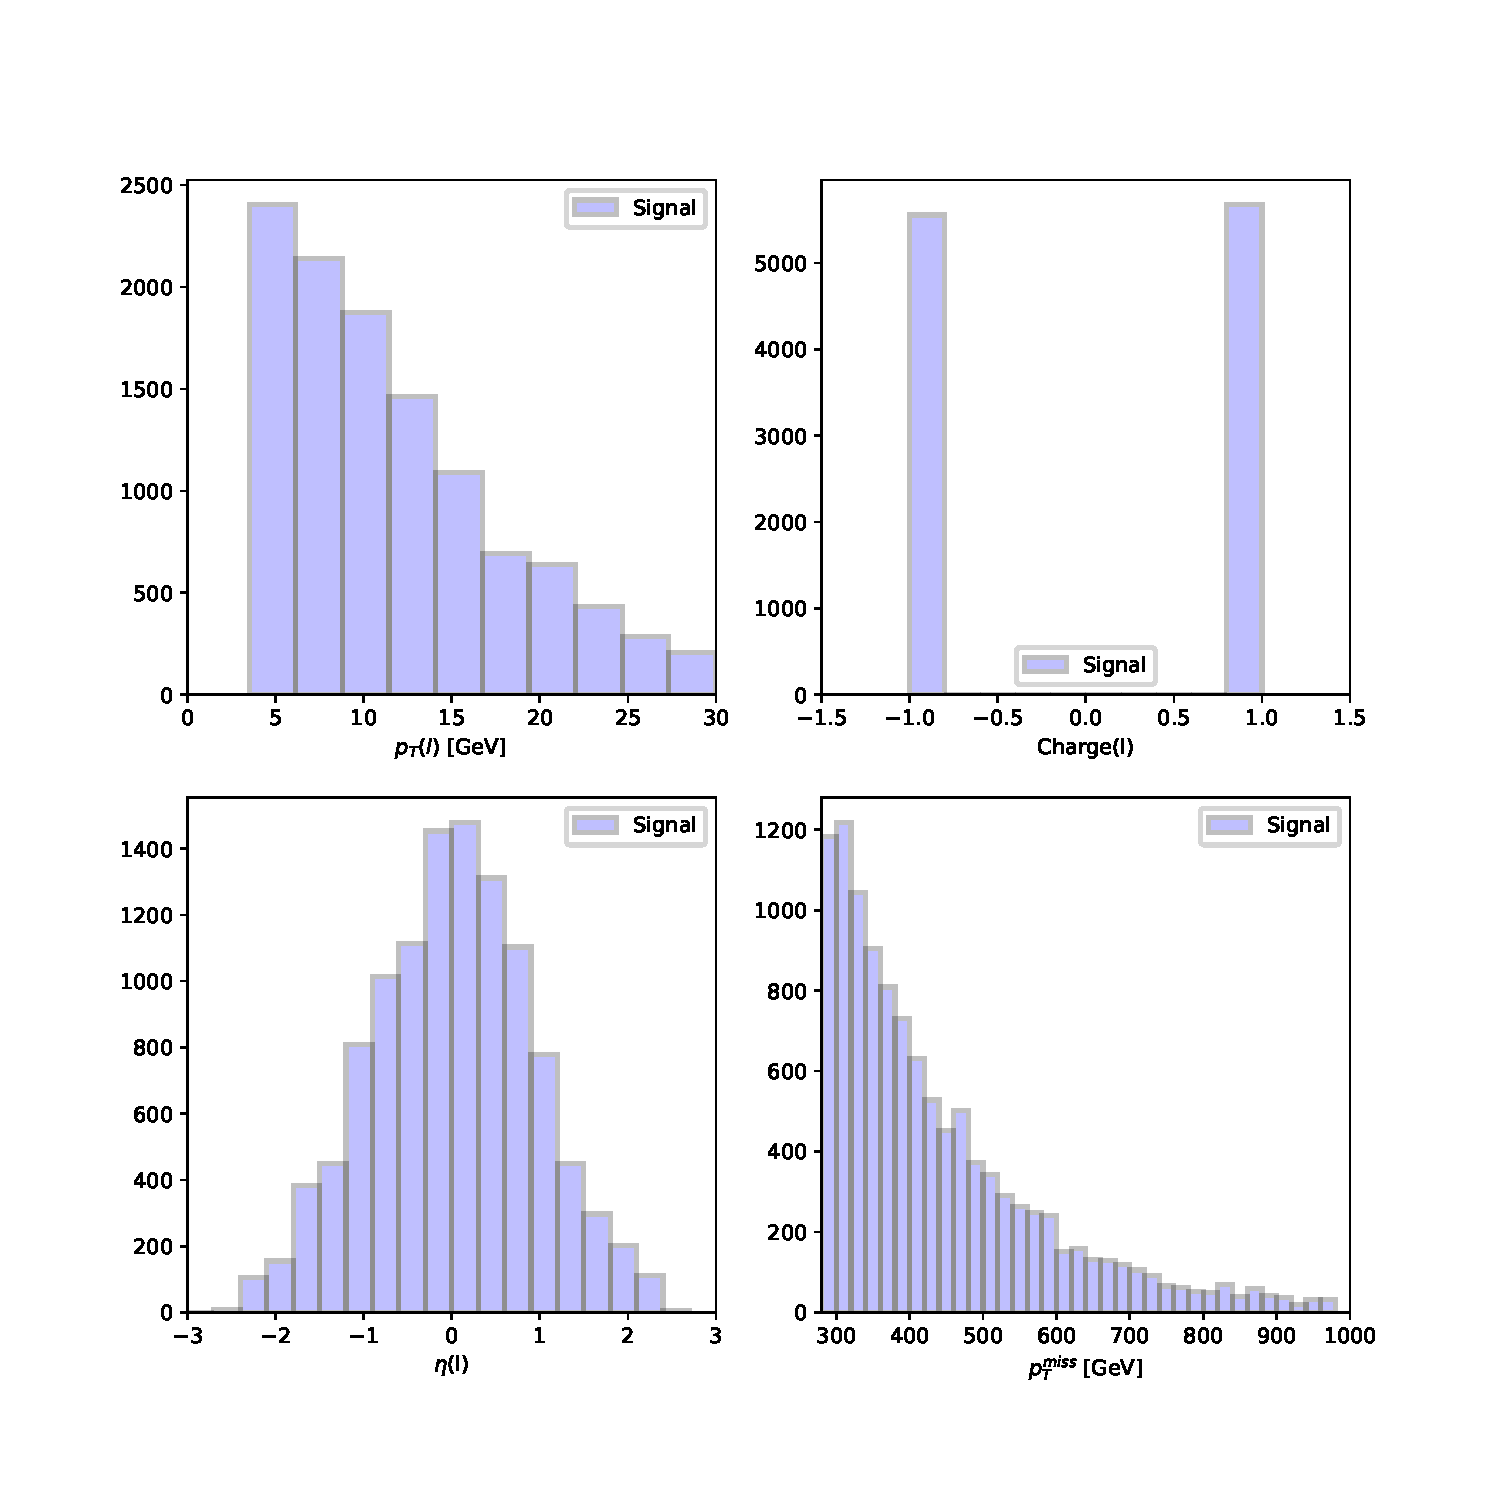
\includegraphics[width=1\textwidth]{figures/features.pdf}
\caption{Distributions of \ptl (upper left), \mt (upper right), \drLB 
    (lower left), and \ptmiss (lower right) after the selection~\ref{eq:presel}.}
\label{fig:features}
\end{figure}

Now that the kinematic variables have been chosen, they have to be transformed
into angles so that later, a qubit is created in a state that translates to the
real value of the distribution. The \ptl and \drLB are transformed into $\eta$
angles, and \mt and \ptmiss are transformed into $\phi$ angles according to 
Figure~\ref{fig:bloch}. The transformed variables are shown in 
Figure~\ref{fig:features_transformed}.

\begin{figure}[!htbp]
\centering
    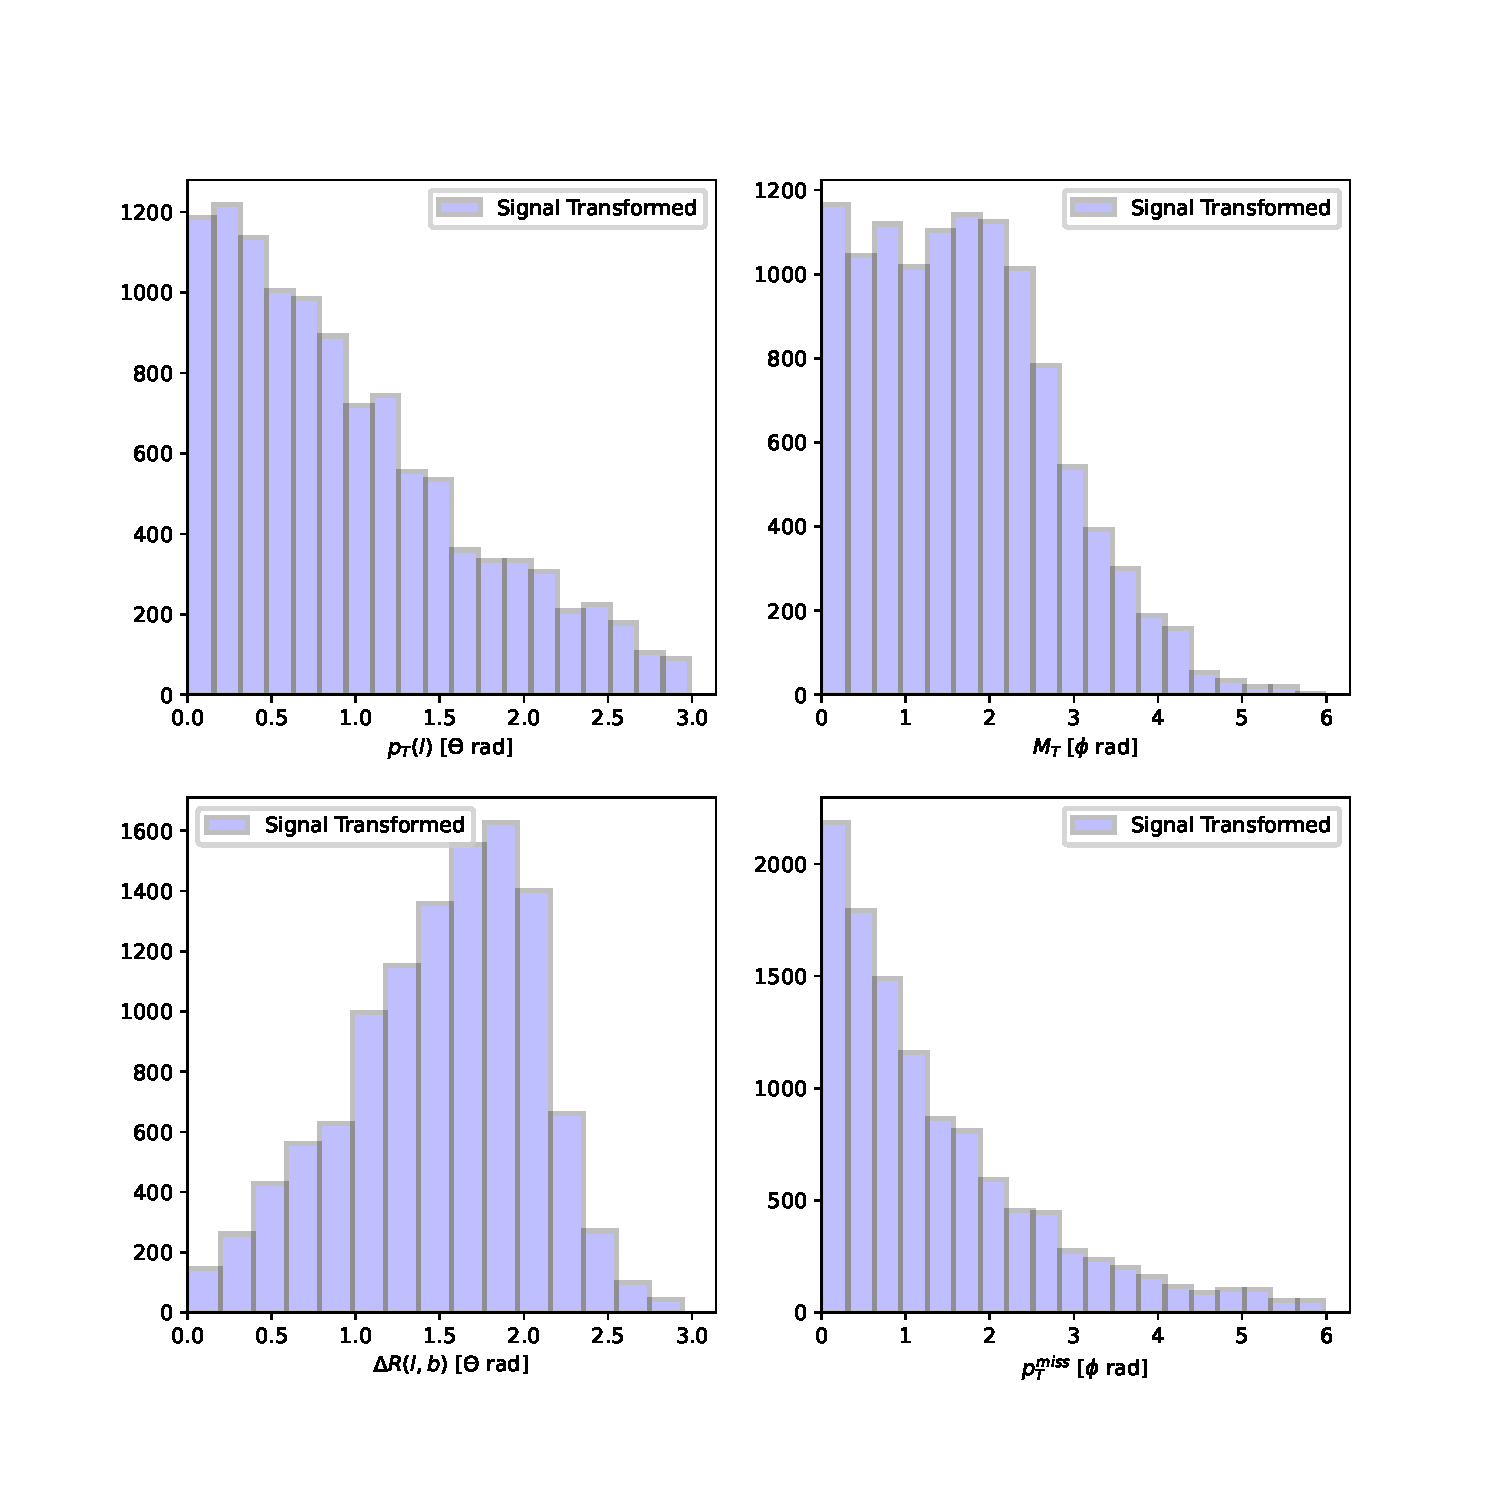
\includegraphics[width=1\textwidth]{figures/features_transformed.pdf}
\caption{Distributions of \ptl (upper left), \mt (upper right), \drLB 
    (lower left), and \ptmiss (lower right) after the angle transformation is 
    applied.}
\label{fig:features_transformed}
\end{figure}

Finally, all the events in the signal samples are translated into state vectors
of two qubits. Qubit 0 is prepared to encode the \ptl and \mt of a given
event and qubit 1 is prepared to encode \drLB and \ptmiss. 
Figure~\ref{fig:features_qubits} helps to visualize this.

\begin{figure}[!htbp]
\centering
    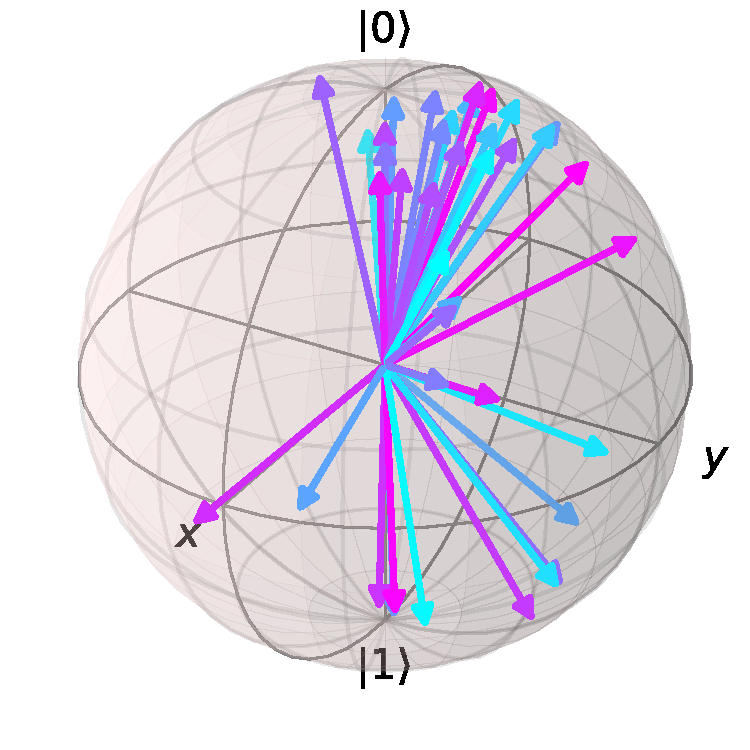
\includegraphics[width=0.49\textwidth]{../assets_dev/bloch1.pdf}
    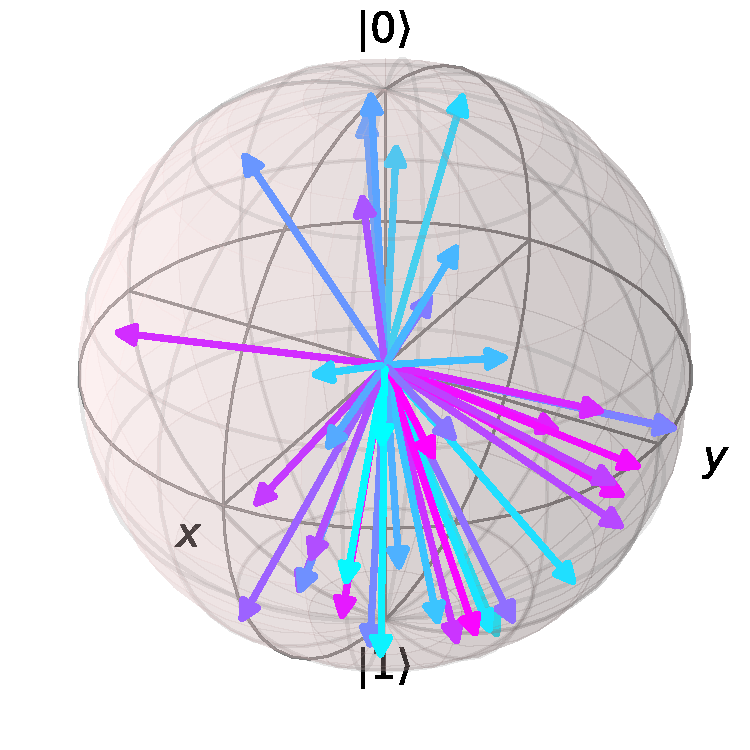
\includegraphics[width=0.49\textwidth]{../assets_dev/bloch2.pdf} \\
    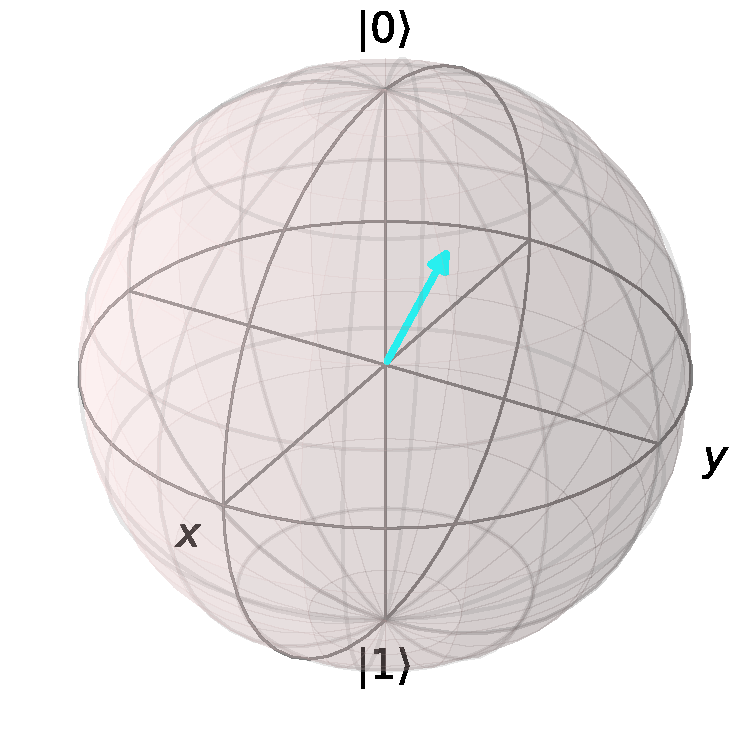
\includegraphics[width=0.49\textwidth]{../assets_dev/bloch_event0_1.pdf}
    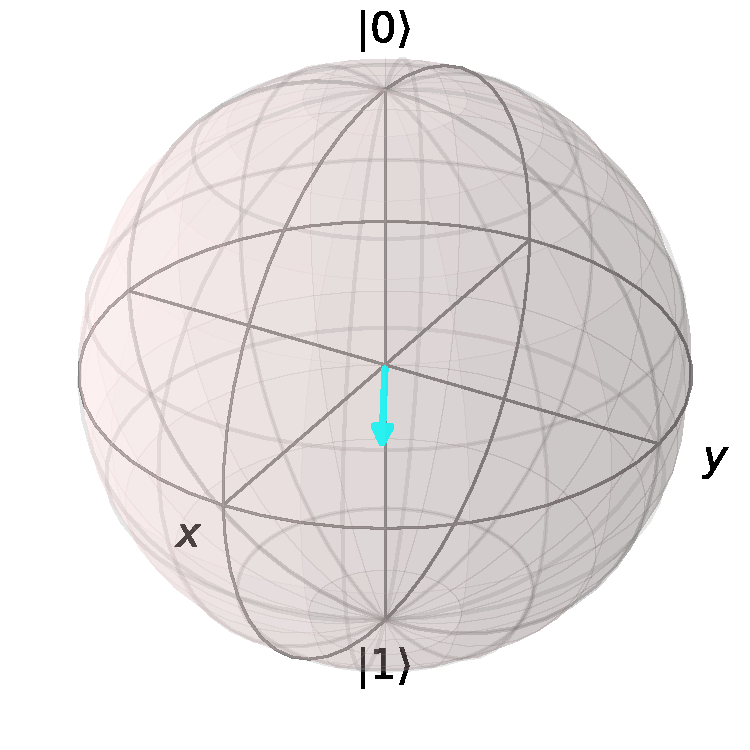
\includegraphics[width=0.49\textwidth]{../assets_dev/bloch_event0_2.pdf} \\
\caption{On top: all the possible states of qubit 0 and qubit 1. On the bottom,
the example of a single signal event in qubit 0 and qubit 1.}
\label{fig:features_qubits}
\end{figure}

Another limitation to running this project in a simulated quantum computer, is
the number of events that can be trained on and generated. From now on, this
project focus on learning the collective state of qubit 0 and qubit 1 of a 
single event and generating a synthetic state of two qubits that could represent
the initial signal sample. Ideally, this algorithm would be deployed on a quantum
computer for every event. This will be discussed in Section~\ref{sec:res}.

\subsection{Designing a qGAN}
\label{sec:qgan}

Given that this section is focused on the design of the \gls{qgan}, python code 
snippets will be shared for a comprehensive and complete description of the 
necessary tools to reproduce the project results.

The first step is to load the necessary python libraries:
\begin{python}
import pennylane as qml
import tensorflow as tf
\end{python}

A 5-qubit simulator device running in Cirq is used to design the \gls{qgan}. Each
of the qubits has a role in the algorithm. The roles are:
\begin{itemize}
    \item Qubits \textbf{0} and \textbf{1}: the 2-qubit state that we are trying
    to generate
    \item Qubits \textbf{2} and \textbf{3}: the generator's playground
    \item Qubit \textbf{4}: the discriminator's guess
\end{itemize}

The 5-qubit simulator quantum device is created by doing the following:

\begin{python}
dev = qml.device('cirq.simulator', wires=5)
\end{python}

The $real$ function uses the angles determined in Section~\ref{sec:prep} and 
rotates the qubits 0 and 1 in state $\vert 0 \rangle$ to the desired position 
reflecting the kinematics of the event:
\begin{python}
angles=[lepPt_to_theta[event],
        mt_to_phi[event],
        DrJetHBLep_to_eta[event],
        Met_to_phi[event]]

def real(angles, **kwargs):
    qml.RY(angles[0], wires=0)
    qml.RZ(angles[1], wires=0)
    qml.RY(angles[2], wires=1)
    qml.RZ(angles[3], wires=1)
\end{python}

\subsection{Discriminator}
\label{sec:disc}

A quantum discriminator is designed in the same manner as an artificial Neural
Network: a first layer to encode the data, a number of hidden layers with a 
trainable parameter and an output layer for the prediction that is going to be 
used in the cost function we want to minimize. Figure~\ref{fig:disc} illustrates
the design of the quantum circuit discriminator.

\begin{figure}[!htbp]
\centering
    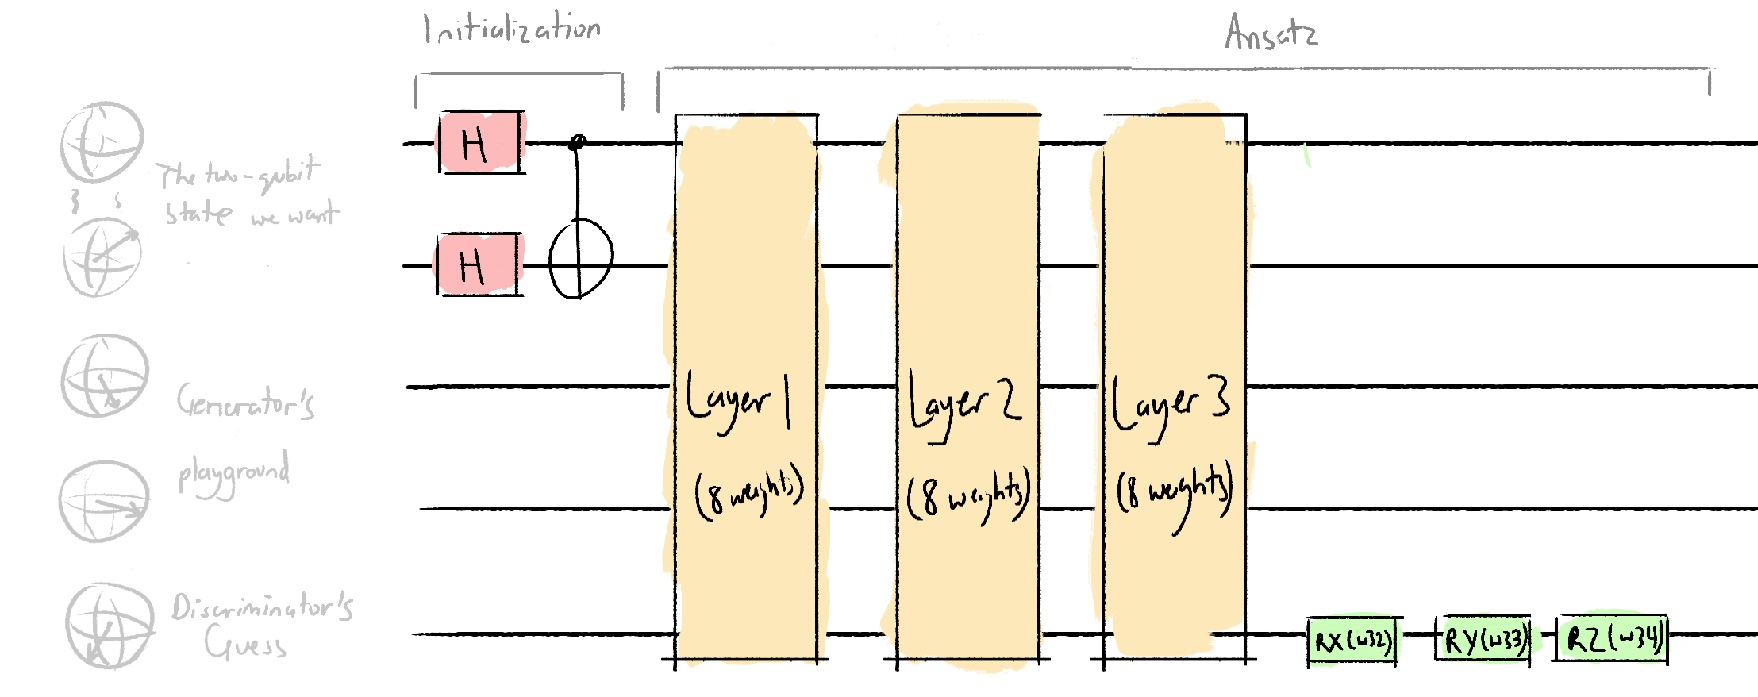
\includegraphics[width=1\textwidth]{figures/discriminator.pdf}
\caption{Design of the quantum discriminator.}
\label{fig:disc}
\end{figure}

The $input\_layer$ ensures that both qubit 0 and 1 are in a superposition and 
entangled. The $hidden\_layer$ receive a weight (an angle) that manipulates 
rotations to the qubits in order to find the best set of angles that can properly
distinguish between real and synthetic data. The $output\_layer$ rotates qubit 4
in all 3 axis before the output which will be the prediction of the discriminator.
Finally, the $discriminator$ circuit is defined as:
\begin{python}
def hidden_layer(w, **kwargs):
    qml.RX(w[0], wires=0)
    qml.RX(w[1], wires=1)
    qml.RX(w[2], wires=4)
    qml.RZ(w[3], wires=0)
    qml.RZ(w[4], wires=1)
    qml.RZ(w[5], wires=4)
    qml.MultiRZ(w[6], wires=[0, 1])
    qml.MultiRZ(w[7], wires=[1, 4])

def discriminator(w, **kwargs):
    # input_layer
    qml.Hadamard(wires=0)
    qml.Hadamard(wires=1)
    qml.CNOT(wires=[0,1])
    # 3 hidden_layers
    hidden_layer(w[:8])
    hidden_layer(w[8:16]) 
    hidden_layer(w[16:24])
    # output_layer
    qml.RX(w[24], wires=4)
    qml.RY(w[25], wires=4)
    qml.RZ(w[26], wires=4)
\end{python}

\subsection{Generator}
\label{sec:gen}

The generator is a \gls{qnn} that does not receive input data but outputs a 2 
qubit state in qubits 0 and 1. It also has hidden layers that depend on weights.
These weights will be optimized in order to "trick" the discriminator to think 
that the data generated is real data. Figure~\ref{fig:gen} illustrates the 
design of the quantum circuit generator.

\begin{figure}[!htbp]
\centering
    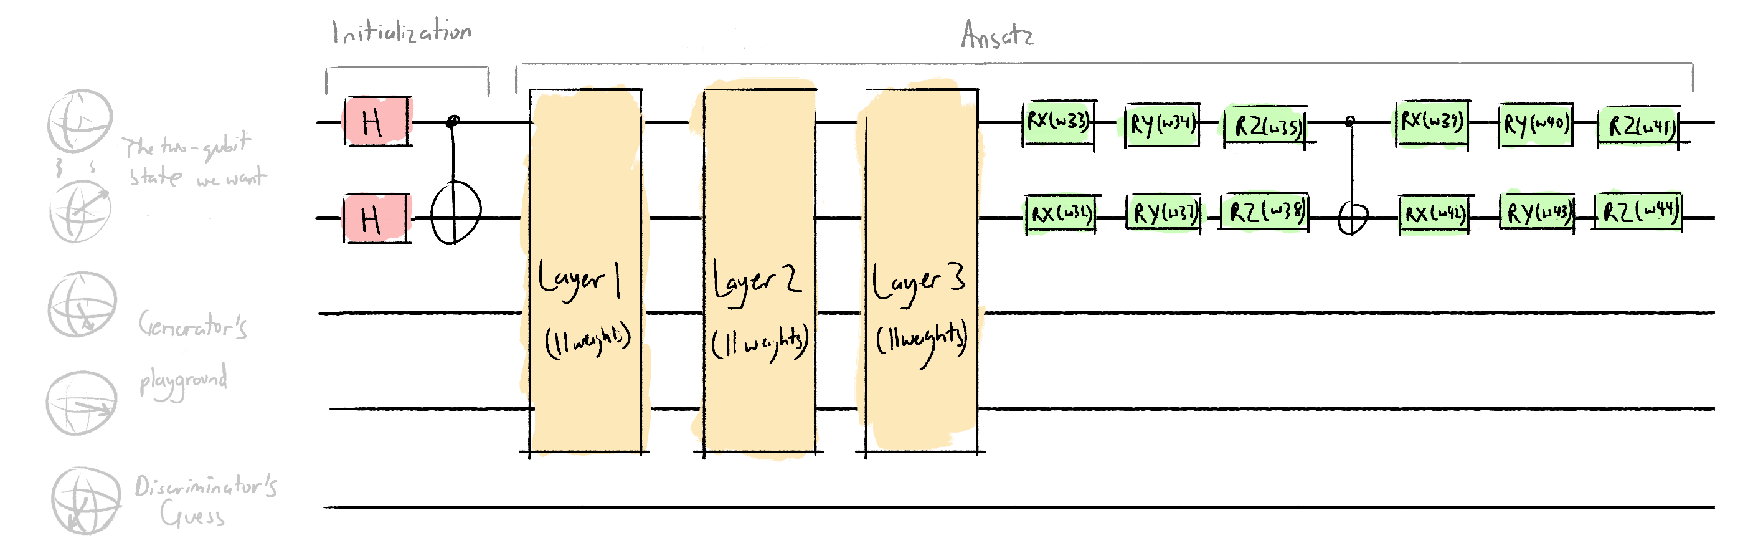
\includegraphics[width=1\textwidth]{figures/generator.pdf}
\caption{Design of the quantum generator.}
\label{fig:gen}
\end{figure}


The $first\_layer$ of the generator ensures that both qubit 0 and 1 in a 
superposition and entangled. The architecture for the $generator\_layer$ is based 
on~\cite{generator}. The $output\_layer$ rotates qubit 0 and 1 in all 3 axis,
entangles them, and rotates them once again. This final state of qubit 0 and 1
corresponds to the synthetic that will be fed to the discriminator. Finally, the
$generator$ circuit is defined as:
\begin{python}
def generator_layer(w):
    qml.RY(w[0], wires=0)
    qml.RY(w[1], wires=1)
    qml.RY(w[2], wires=2)
    qml.RY(w[3], wires=3)
    qml.RZ(w[4], wires=0)
    qml.RZ(w[5], wires=1)
    qml.RZ(w[6], wires=2)
    qml.RZ(w[7], wires=3)
    qml.MultiRZ(w[8], wires=[0, 1])
    qml.MultiRZ(w[9], wires=[2, 3])
    qml.MultiRZ(w[10], wires=[1, 2])

def generator(w, **kwargs):
    # first_layer
    qml.Hadamard(wires=0)
    qml.Hadamard(wires=1)
    qml.CNOT(wires=[0,1])
    qml.Barrier(wires=[0,4],only_visual=True)
    # 3 generator lawyers
    generator_layer(w[:11])
    generator_layer(w[11:22])
    generator_layer(w[22:33])
    # output_layer
    qml.RX(w[33], wires=0)
    qml.RY(w[34], wires=0)
    qml.RZ(w[35], wires=0)
    qml.RX(w[36], wires=1)
    qml.RY(w[37], wires=1)
    qml.RZ(w[38], wires=1)
    qml.CNOT(wires=[0, 1])
    qml.RX(w[39], wires=0)
    qml.RY(w[40], wires=0)
    qml.RZ(w[41], wires=0)
    qml.RX(w[42], wires=1)
    qml.RY(w[43], wires=1)
    qml.RZ(w[44], wires=1)
\end{python}

\subsection{Quantum nodes}
\label{sec:qnode}

A $QNode$ contains a quantum function and the computational device it is 
executed on. We need to create two quantum nodes. One to train the discriminator,
we feed the real data to the discriminator so that it can learn it. A second one
where we feed generated data to train the generator.
\begin{python}
@qml.qnode(dev, interface='tf')
def real_disc_circuit(angles, disc_weights):
    real(angles)
    discriminator(disc_weights)
    return qml.expval(qml.PauliZ(4))

@qml.qnode(dev, interface='tf')
def gen_disc_circuit(gen_weights, disc_weights):
    generator(gen_weights)
    discriminator(disc_weights)
    return qml.expval(qml.PauliZ(4)) 
\end{python}

Figure~\ref{fig:real_disc_cirq} illustrates the real+discriminator quantum 
circuit.

\begin{figure}[!htbp]
\centering
    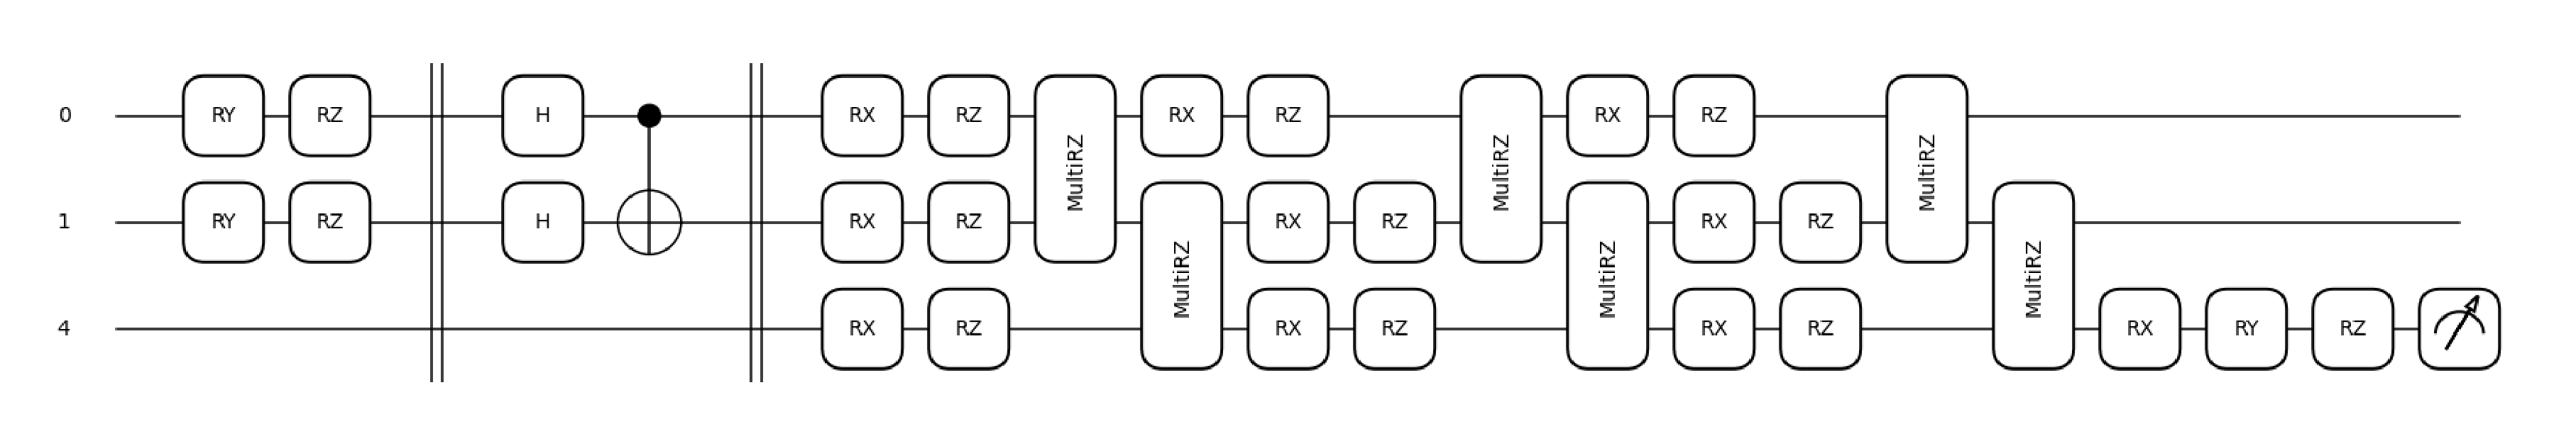
\includegraphics[width=1\textwidth]{figures/real_disc_cirq.pdf}
\caption{Real+discriminator quantum circuit.}
\label{fig:real_disc_cirq}
\end{figure}

Figure~\ref{fig:gen_disc_cirq} illustrates the generator+discriminator quantum 
circuit.

\begin{figure}[!htbp]
\centering
    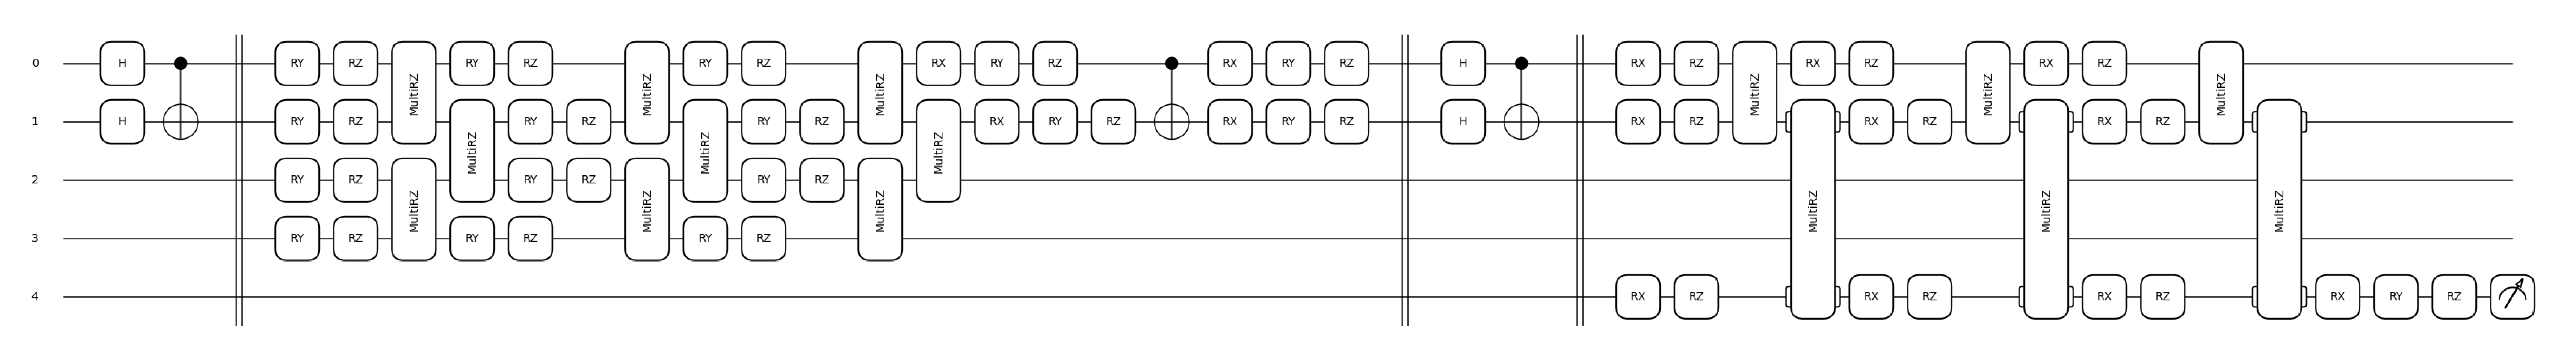
\includegraphics[width=1\textwidth]{figures/gen_disc_cirq.pdf}
\caption{Generator quantum circuit.}
\label{fig:gen_disc_cirq}
\end{figure}

\subsection{Cost Functions}
\label{sec:cost}

There are two cost functions of interest, corresponding to the two stages of 
the \gls{qgan} training. These cost functions are built in two parts: the 
first part is the probability that the discriminator correctly classifies real 
data as real (true). The second piece is the probability that the discriminator 
classifies generated data as real.

The discriminator is trained to maximize the probability of correctly classifying 
real data, while minimizing the probability of mistakenly classifying gen data:

\begin{linenomath}
\begin{equation}
Cost_D=Prob(true|\mathrm{gen})-Prob(true|\mathrm{real})
\label{eq:costd}
\end{equation}
\end{linenomath}

The generator is trained to maximize the probability that the discriminator 
accepts generated data as real:

\begin{linenomath}
\begin{equation}
Cost_G=-Prob(true|\mathrm{gen})
\label{eq:costg}
\end{equation}
\end{linenomath}

In code format:
\begin{python}
def prob_real_true(disc_weights):
    true_disc_output = real_disc_circuit(phi, theta, omega, disc_weights)
    # convert to probability
    prob_real_true = (true_disc_output + 1) / 2
    return prob_real_true

def prob_gen_true(gen_weights, disc_weights):
    gen_disc_output = gen_disc_circuit(gen_weights, disc_weights)
    # convert to probability
    prob_gen_true = (gen_disc_output + 1) / 2
    return prob_gen_true

def disc_cost(disc_weights):
    cost = prob_gen_true(gen_weights, disc_weights) - 
        prob_real_true(disc_weights)
    return cost

def gen_cost(gen_weights):
    return -prob_gen_true(gen_weights, disc_weights)
\end{python}

\subsection{Training: Discriminator vs Generator}
\label{sec:vs}

Both the initial weights for the discriminator and the generator are randomly
initialized. 
%At this level, the probability for the discriminator to classify 
%real data as true is $\approx$8\% and the probability to classify generated 
%data as true is $\approx$58\%. 
The Stochastic Gradient Descent Optimizer~\cite{SGC} is used to minimize both 
cost functions and find the best discriminator and generator weights. Next,
the training functions are defined:
\begin{python}
opt = tf.keras.optimizers.SGD(0.4)

def train_disc(it,disc_loss):
    cost = lambda: disc_cost(disc_weights)
    for step in range(it+1):
        opt.minimize(cost, disc_weights) 

def train_gen(it,gen_loss):
    cost = lambda: gen_cost(gen_weights)
    for step in range(it+1):
        opt.minimize(cost, gen_weights)
\end{python}

The complete train of the \gls{qgan} consists in repeating 7 times a training 
cycle. A training cycle is defined by training the discriminator followed by 
training the generator.
At the end of the complete train, the probability for the discriminator to 
classify real data as true is $\approx$75\% and the probability to classify 
generated data as true is $\approx$99\%. A complete train takes $\approx$35 
minutes in my personal computer, this for a single event.

\begin{figure}[!htbp]
\centering
    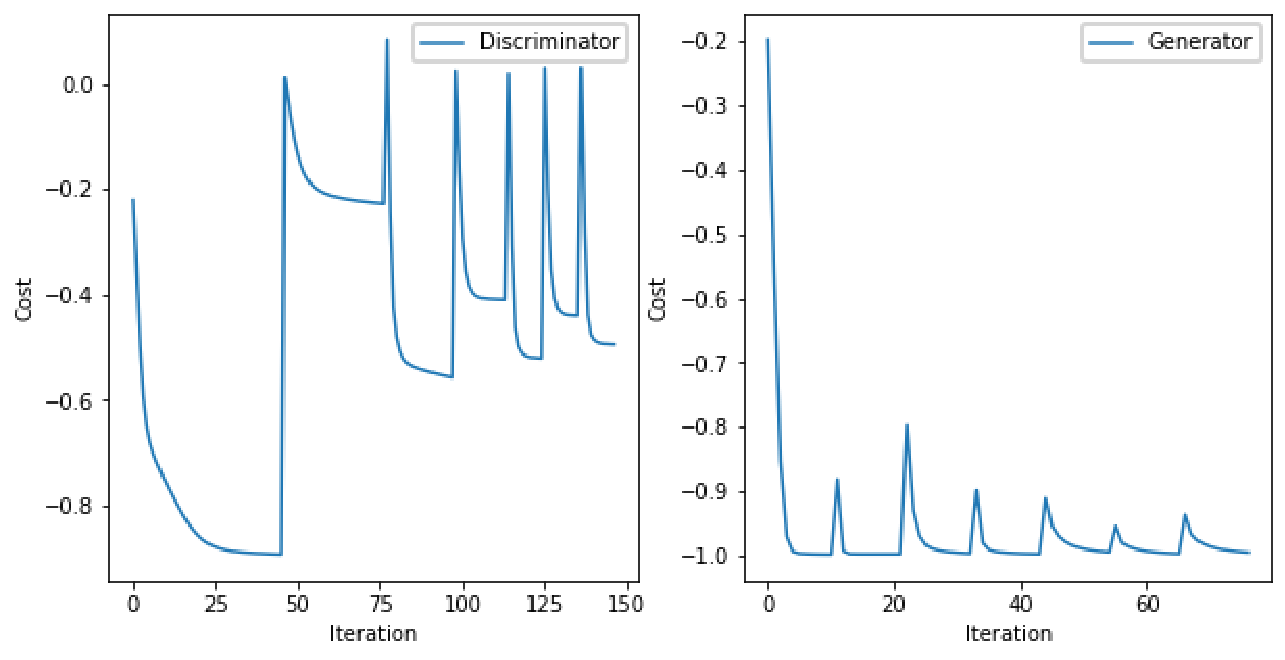
\includegraphics[width=1\textwidth]{figures/costs.pdf}
\caption{The cost for both the discriminator and generator as a function of 
        number of iterations.}
\label{fig:costs}
\end{figure}

\subsection{Results}
\label{sec:res}

We can now compare the real data with the generated one in Figure~\ref{fig:bloschres} 
and transform the generated qubits into the generated events kinematics. The 
latter is reported in Table~\ref{tab:res}.

\begin{figure}[!htbp]
\centering
    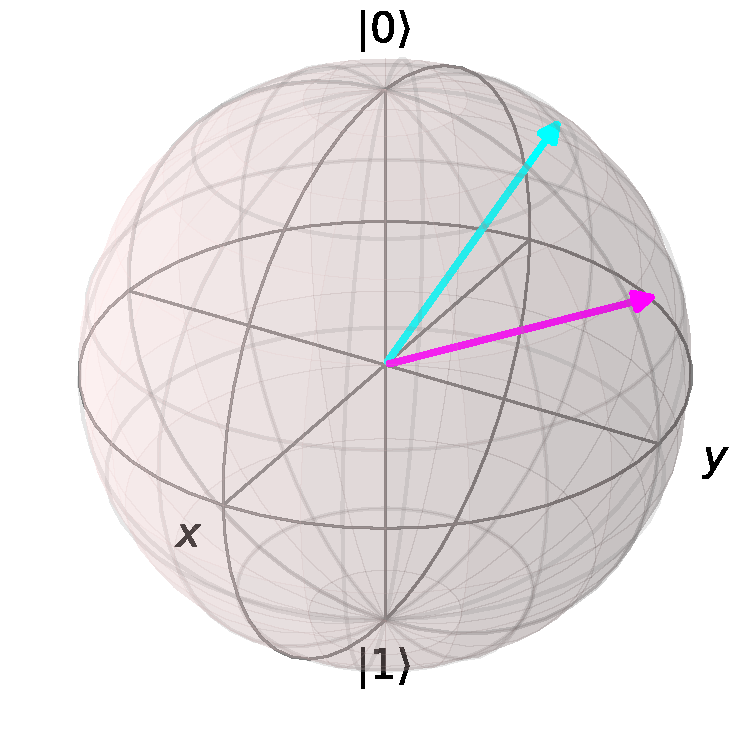
\includegraphics[width=0.43\textwidth]{../results_7C/1360_Q1.pdf}
    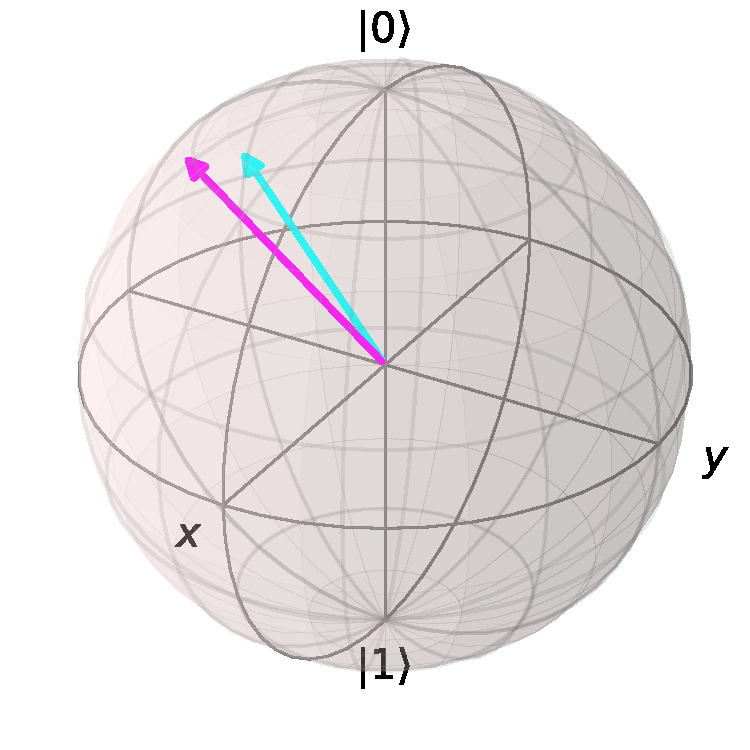
\includegraphics[width=0.43\textwidth]{../results_7C/1360_Q2.pdf} \\
    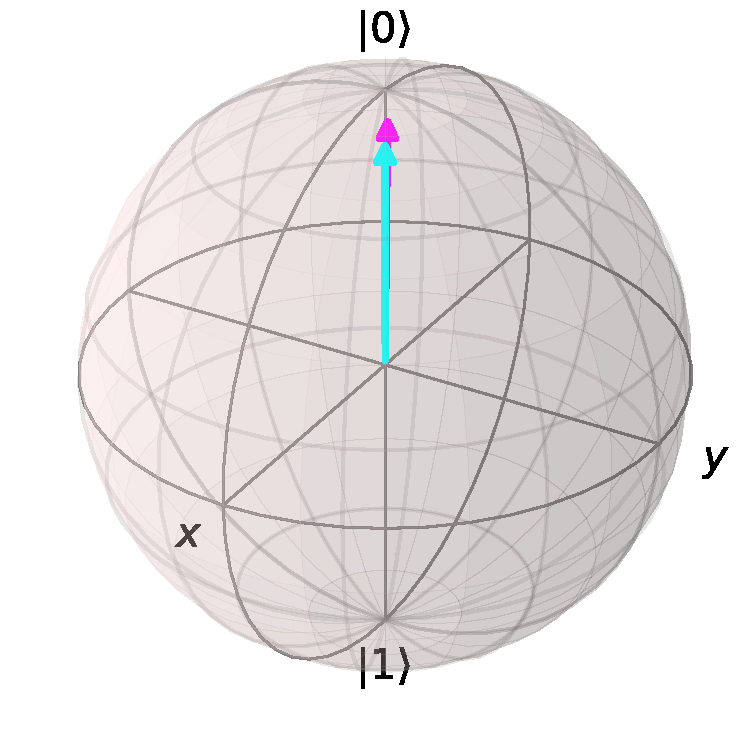
\includegraphics[width=0.43\textwidth]{../results_7C/1785_Q1.pdf}
    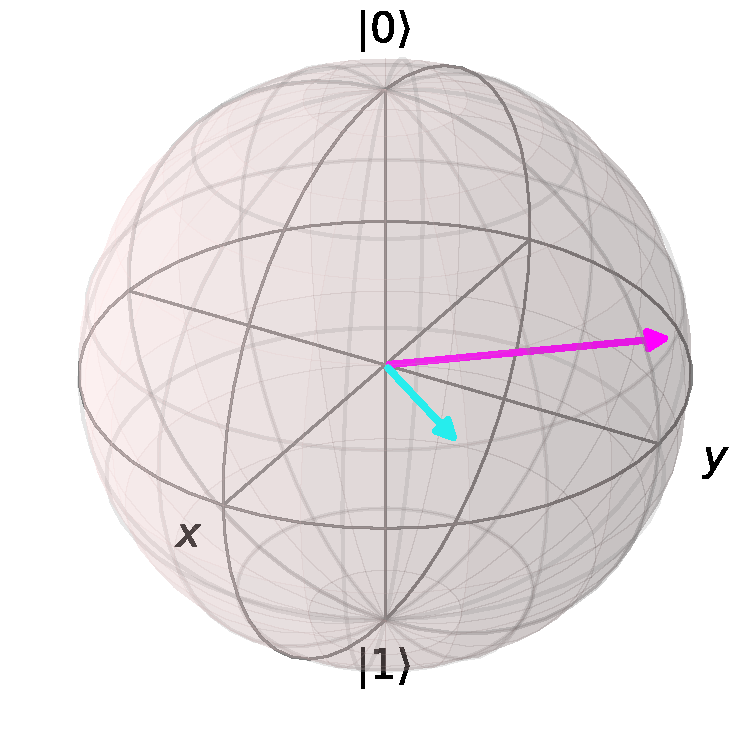
\includegraphics[width=0.43\textwidth]{../results_7C/1785_Q2.pdf} \\
    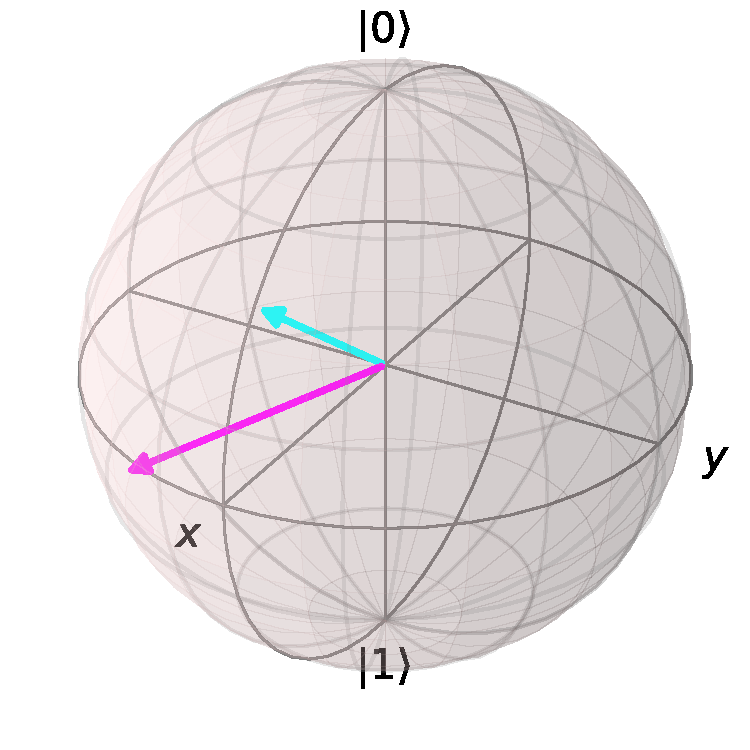
\includegraphics[width=0.43\textwidth]{../results_7C/3400_Q1.pdf}
    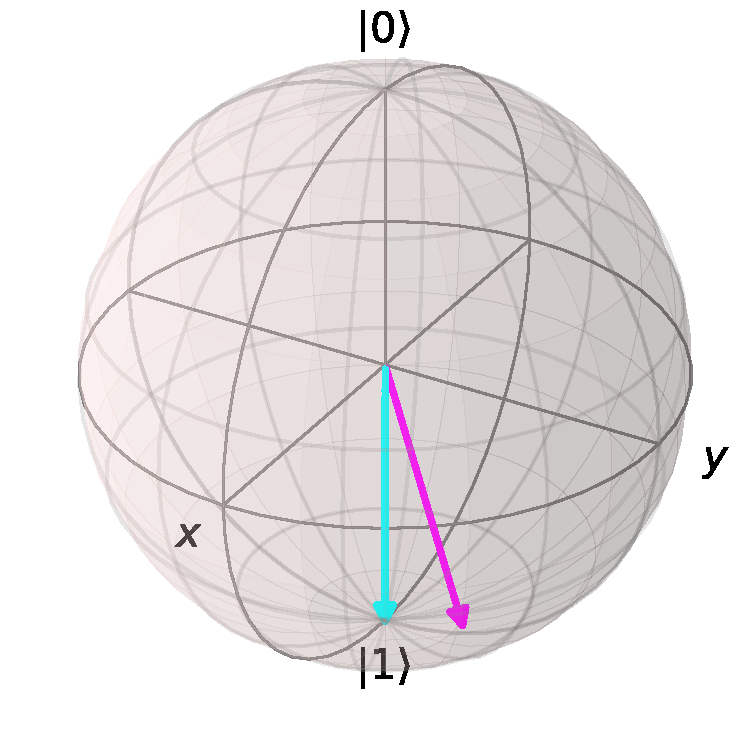
\includegraphics[width=0.43\textwidth]{../results_7C/3400_Q2.pdf} \\
\caption{Comparison in the Bloch sphere of the real data (in blue) with the 
        generated one (in pink) for both qubits 0 and 1.}
\label{fig:bloschres}
\end{figure}

\begin{table}[!htbp]
\centering
\caption{Comparison of the event kinematics between the real and generated 
        events reported in Figure~\ref{fig:bloschres}.}
\begin{tabular}{lcccc}
Data      & \ptl [GeV] & \mt [GeV] & \drLB & \ptmiss [GeV] \\
\hline
real   & 9.9   & 101.5 & 1.8 & 514.15 \\
fake   & 13.7   & 72.8 & 1.5 & 458.85 \\
\hline
real      & 5.6   & 20 & 2.0 & 368 \\
generated & 5.3   & 23 & 2.1 & 493 \\
\hline
real      & 18.9   & 81 & 3.1 & 340 \\
generated & 20.6   & 42 & 3.3 & 377 \\ 
\end{tabular}
\label{tab:res}
\end{table}

